%% horizontal_self_org.tex
This chapter presents a method based on horizontal self-organisation (c.f. \secref{neuro_concepts_self_org}).
The idea of horizontal self-organisation is that the input is analysed by several smaller models instead of one big model.
This means that each network sees only a patch of the input data and cannot decide on its own what is represented in the input image, but must agree on a representation with neighbouring models.
It is important that each model is independent of the other models and that the parameters are not shared between the models. Otherwise the architecture would be comparable to vision transformer \sidecite{Dosovitskiy_Beyer_Kolesnikov_Weissenborn_Zhai_Unterthiner_Dehghani_Minderer_Heigold_Gelly_2021} and the input patches would no longer be analysed independently.


In the following, first the methodology (i.e. how horizontal self-organization is implemented) is presented and afterwards the obtained results are discussed in detail.


\section{Methods}\seclbl{horizontal_self_org_methods}
A crucial design-decision for horizontal self-organisation is the architecture of the models.
In this thesis are variational auto-encoders \sidecite{Kingma_Welling_2014} (c.f. \secref{visual_rep_learning}) used to process patches of the input image as they have a continuous latent space and are thus more robust and better interpretable (c.f. \secref{neuro_concepts_net_fragments}).

Typical auto-encoders fed an input image $\boldsymbol{x}$ through an encoder to map the input data to a latent space and through a decoder to recreate the image $\boldsymbol{\hat{x}}$. Thereby, the latent space is limited in size, forcing the model to compress the image with the encoder and to de-compress the image using the decoder.

A variational auto-encoder models the latent space as a multivariate Gaussian distribution. The input image $\boldsymbol{x}$ is also fed through a encoder and a latent representation $\boldsymbol{z}$ is obtained. Afterwards, $\boldsymbol{z}$ is fed through two independent parallel fully connected layers to obtain the $\boldsymbol{\mu}$ and $\boldsymbol{\sigma}$ vectors of the multivariate Gaussian distribution. Afterwards, the re-parametrization trick is used to sample a variable $\boldsymbol{z}'$ from this distribution:

\begin{equation}\eqlbl{hso_1}
	\boldsymbol{z}' \sim \mathcal{N}(\boldsymbol{\mu},\,\boldsymbol{\sigma}^{2} \cdot \epsilon)
\end{equation}

$\epsilon$ is a random variable sampled from  $\mathcal{N}(0, 1)$ and determines the magnitude of the variance. The sampled latent representation is then fed through the decoder and the image $\hat{\boldsymbol{x}}$ is recreated. The model is trained to minimize a distance measure between the input image $\boldsymbol{x}$ and the reconstructed image $\hat{\boldsymbol{x}}$. In this thesis, the mean square error is used. For $n$ images $\boldsymbol{X} = \boldsymbol{x}_1, ..., \boldsymbol{x}_n$, the loss is defined as

\begin{equation}\eqlbl{hso_2}
	L_{\text{reconstruction}} = \frac{1}{n} \sum_{i=1}^{n} (\boldsymbol{x}_i - \boldsymbol{\hat{x}}_i)^2
\end{equation}

However, the latent space does not form a multivariate Gaussian distribution on the basis of this reconstruction loss and the network architecture. To accomplish this, a second loss constraint is necessary: Let $P(\boldsymbol{X})$ be the probability distribution of the data $\boldsymbol{X}$, $P(\boldsymbol{z})$ the probability distribution of the latent variable $\boldsymbol{z}$ and $P(\boldsymbol{X}|\boldsymbol{z})$ the probability distribution of generating $\boldsymbol{X}$ for a given $\boldsymbol{z}$. The objective of the VAE is to infer $P(\boldsymbol{z})$ from $P(\boldsymbol{z}|\boldsymbol{X})$ which is the probability distribution that maps $\boldsymbol{X}$ into latent space. Simply put: we want to know what the latent variable $\boldsymbol{z}$ of the input data $\boldsymbol{X}$ is.
However, $P(\boldsymbol{z}|\boldsymbol{X})$ is unknown and we have to estimate it from a simpler distribution $Q(\boldsymbol{z}|\boldsymbol{X})$. This simpler distribution $Q(\boldsymbol{z}|\boldsymbol{X})$ is learned by the encoder and should be as close as possible to the real distribution $P(\boldsymbol{z}|\boldsymbol{X})$. This is accomplished by minimizing the KL divergence\sidenote{the Kullback-Leibler (KL) divergence can ``measure'' the difference between two probability distributions} between these two probability distributions.

\begin{equation}\eqlbl{hso_3}
	KL \left[ Q(\boldsymbol{z}|\boldsymbol{X}) || P(\boldsymbol{z}|\boldsymbol{X}) \right] = E \left[ \log Q(\boldsymbol{z}|\boldsymbol{X}) - \log P(\boldsymbol{z}|\boldsymbol{X}) \right]
\end{equation}

In case of two Gaussian distributions, the KL divergence is defined as:
\begin{equation}\eqlbl{hso_4}
	KL\left[ \mathcal{N}_Q(\boldsymbol{\mu}_Q, \boldsymbol{\sigma}_Q)||\mathcal{N}_P(\boldsymbol{\mu}_P, \boldsymbol{\sigma}_P) \right] = \log \frac{\boldsymbol{\sigma}_P}{\boldsymbol{\sigma}_Q} + \frac{\boldsymbol{\sigma}_Q^2 + (\boldsymbol{\mu}_Q-\boldsymbol{\mu}_P)^2}{2\boldsymbol{\sigma}_P^2} - \frac{1}{2}
\end{equation}


If the target distribution $P(\boldsymbol{z}|\boldsymbol{X})$ is a multivariate Gaussian distribution with $\boldsymbol{\mu}_P = 0$ and $\boldsymbol{\sigma}_P=1$ (i.e. $\mathcal{N}(0, 1)$) and the encoder predicts $\boldsymbol{\mu}_Q$ and $\boldsymbol{\sigma}_Q$ to model $Q(\boldsymbol{z}|\boldsymbol{X})$ as $\mathcal{N}(\boldsymbol{\mu}_Q, \boldsymbol{\sigma}_Q)$, then the KL divergence simplifies to


\begin{equation*}\eqlbl{hso_5}
\begin{split}
		L_{KLD} = KL \left[ \mathcal{N}_Q(\boldsymbol{\mu}_Q, \boldsymbol{\sigma}_Q)||\mathcal{N}(0, 1) \right] & = -\log \boldsymbol{\sigma}_Q + \frac{\boldsymbol{\sigma}_Q^2 \boldsymbol{\mu}_Q^2}{2} - \frac{1}{2} \\
		 & = \frac{1}{2} \left( \boldsymbol{\sigma}_Q^2 \boldsymbol{\mu}_Q^2 - 1 - 2\log \boldsymbol{\sigma}_Q \right)
\end{split}
\end{equation*}

Interested reads may find a formal proof of the formulas above and a more detailed derivation in the original paper \cite{Kingma_Welling_2014}.
Thus, the loss for the variational auto-encoder is defined as:


\begin{equation*}\eqlbl{hso_6}
\begin{split}
		L_{\text{VAE}} & = L_{\text{reconstruction}} + \beta \cdot KL \left[ \mathcal{N}_Q(\boldsymbol{\mu}_Q, \boldsymbol{\sigma}_Q)||\mathcal{N}(0, 1) \right] \\
		  & = \underbrace{\frac{1}{n} \sum_{i=1}^{n} (\boldsymbol{x}_i - \boldsymbol{\hat{x}}_i)^2}_{\text{reconstruction loss}} + \lambda \cdot \overbrace{\frac{1}{2} (\boldsymbol{\sigma}_Q^2 \boldsymbol{\mu}_Q^2 - 1 - 2\log \boldsymbol{\sigma}_Q)}^{\text{KL divergence}}
\end{split}
\end{equation*}

where $\beta$ is a factor to weight the KL divergence. Training an variational auto-encoder with this loss functions can lead to very good reconstructions.
In the case of horizontal self-organisation, however, a well-formed latent space is of more interest than a excellent image reconstruction: Latent representations are extracted from the latent space and made available to neighbouring models. Based on these latent representations, multiple variational auto-encoders should agree on a suitable image representation.
Variational auto-encoders have the notorious problem that the KL divergence term becomes vanishingly small during training \sidecite{bowman2016generating}. This issue is known as the KL vanishing problem.
This problem can be alleviated by applying annealing schedules to the KL term (i.e. by changing $\beta$ over time).
In this thesis, monotonic annealing is used as proposed by Ref. \cite{bowman2016generating} since this seems sufficient.
However, for a slight increase in computational costs, cyclic annealing strategies might lead to even better results \sidecite{Fu_Li_Liu_Gao_Celikyilmaz_Carin_2019}.
These annealing strategies are shown in Figure \figref{beta_annealing}. When $\beta$ is small, the model is forced to focus on reconstructing the input rather than minimizing the KL loss.
When $\beta$ is increased, the model gradually improves the shape of the data distribution in the latent space.

\begin{figure}[h]
    \centering
    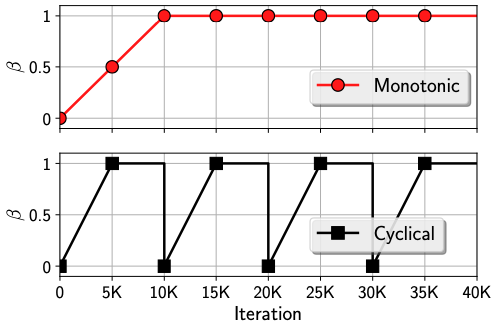
\includegraphics[width=0.5\textwidth]{beta_annealing}
    \caption[Annealing strategy of the KL weight term in variational auto-encoders]{Two annealing strategies for the $\beta$ term that weights the KL divergence in the loss function of variational auto-encoders. The upper graph shows a monotonic increase of $\beta$, the lower graph a cyclical annealing strategy. The picture is from \cite{Fu_Li_Liu_Gao_Celikyilmaz_Carin_2019}.}
    \figlbl{beta_annealing}
\end{figure}


In this thesis, $4$ variational auto-encoders are used. Each VAE consists of an encoder, two fully-connected layers to calculate $\boldsymbol{\mu}$ and $\boldsymbol{\sigma}$, and a decoder.
The encoder consists of $3$  convolutional layers with $32$, $64$, and $128$ channels. Each convolutional layer has a stride of $2$, halving the size of the input in each layer.
The decoder has the inverse structure of the encoder, i.e. $3$ transposed convolutional layers with $128$, $64$, and $32$ channels.
The fully connected layer for predicting $\boldsymbol{\mu}$ and $\boldsymbol{\sigma}$ have $32$ neurons.
The network architecture is shown in Figure \figref{horizontal_org_arch1}.


\begin{figure}[h]
    \centering
    \resizebox{0.99\textwidth}{!}
{
\begin{tikzpicture}
\tikzstyle{connection}=[ultra thick,every node/.style={sloped,allow upside down},draw=\edgecolor,opacity=0.7]
\tikzstyle{copyconnection}=[ultra thick,every node/.style={sloped,allow upside down},draw={rgb:blue,4;red,1;green,1;black,3},opacity=0.7]


\node[canvas is zy plane at x=0] (input) at (0,0,0) {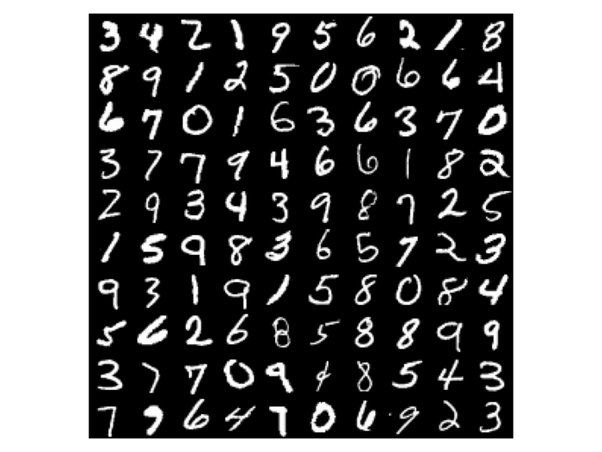
\includegraphics[width=8cm,height=8cm]{imgs/mnist.jpeg}};


\pic[shift={(3,0,0)}] at (input) 
    {Box={
        name=conv1,
        caption=Conv + ReLU,
        xlabel={{1, }},
        zlabel=32,
        fill=\ConvColor,
        height=20,
        width=2,
        depth=20
        }
    };


\draw [connection]  (input) ++(0,0,0)    -- node {\midarrow} (conv1-west);


\pic[shift={(2,0,0)}] at (conv1-east) 
    {Box={
        name=conv2,
        caption=Conv + ReLU,
        xlabel={{32, }},
        zlabel=64,
        fill=\ConvColor,
        height=12,
        width=4,
        depth=12
        }
    };


\draw [connection]  (conv1-east)    -- node {\midarrow} (conv2-west);


\pic[shift={(2,0,0)}] at (conv2-east) 
    {Box={
        name=conv3,
        caption=Conv + ReLU,
        xlabel={{64, }},
        zlabel=128,
        fill=\ConvColor,
        height=6,
        width=6,
        depth=6
        }
    };


\draw [connection]  (conv2-east)    -- node {\midarrow} (conv3-west);


\pic[shift={(2,2,0)}] at (conv3-east) 
    {Box={
        name=fcn1,
        caption=FC + ReLU,
        xlabel={{" ","dummy"}},
        zlabel=32,
        fill=\SoftmaxColor,
        opacity=0.8,
        height=3,
        width=3,
        depth=6
        }
    };


\pic[shift={(2,-2,0)}] at (conv3-east) 
    {Box={
        name=fcn2,
        caption=FC + ReLU,
        xlabel={{" ","dummy"}},
        zlabel=32,
        fill=\SoftmaxColor,
        opacity=0.8,
        height=3,
        width=3,
        depth=6
        }
    };


\draw [connection]  (conv3-east)    -- node {\midarrow} (fcn1-west);


\draw [connection]  (conv3-east)    -- node {\midarrow} (fcn2-west);


\pic[shift={(2,-2,0)}] at (fcn1-east) 
    {Box={
        name=conv4,
        caption=Conv + ReLU,
        xlabel={{128, }},
        zlabel=64,
        fill=\ConvColor,
        height=6,
        width=6,
        depth=6
        }
    };


\draw [connection]  (fcn1-east)    -- node {\midarrow} (conv4-west);


\draw [connection]  (fcn2-east)    -- node {\midarrow} (conv4-west);


\pic[shift={(2,0,0)}] at (conv4-east) 
    {Box={
        name=conv5,
        caption=Conv + ReLU,
        xlabel={{64, }},
        zlabel=32,
        fill=\ConvColor,
        height=12,
        width=4,
        depth=12
        }
    };


\draw [connection]  (conv4-east)    -- node {\midarrow} (conv5-west);


\pic[shift={(2,0,0)}] at (conv5-east) 
    {Box={
        name=conv6,
        caption=Conv + ReLU,
        xlabel={{32, }},
        zlabel=1,
        fill=\ConvColor,
        height=20,
        width=2,
        depth=20
        }
    };


\draw [connection]  (conv5-east)    -- node {\midarrow} (conv6-west);


\node[canvas is zy plane at x=3] (output) at (conv6-east) {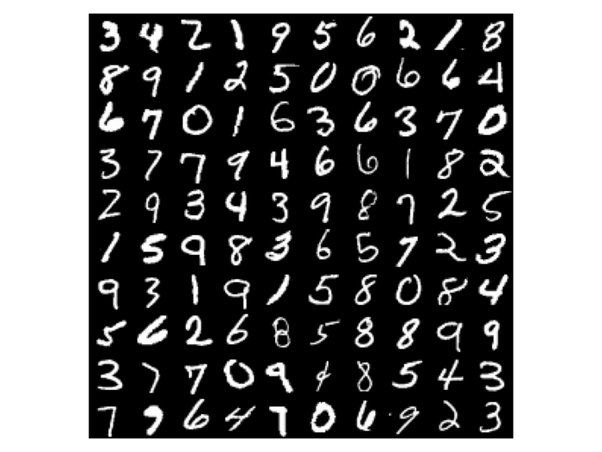
\includegraphics[width=8cm,height=8cm]{imgs/mnist.jpeg}};


\draw [connection]  (conv6-east)     -- node {\midarrow} ($(output) + (0.5,0,0)$);


\end{tikzpicture}
}
    \caption[Architecture of the variational auto-encoder used for horizontal self-organisation]{Architecture of the variational auto-encoder used for horizontal self-organisation.}
    \figlbl{horizontal_org_arch1}
\end{figure}


Each VAE is trained independently with the goal to minimize the loss function as described in \eqref{hso_6}.
Adam \sidecite{Kingma_Ba_2017} is used as optimizer with a learning rate of $1\cdot 10^{-3}$ and the mini-batch size is $32$.



\subsection{Predicting bigger Patches}\seclbl{horizontal_self_org_methods_bigger_patches}
Applying a monotonic annealing to the KL divergence weight term $\beta$ is the first measure to improve the latent space distribution.
Another measure is to predict bigger patches.
The VAEs have a very limited field of view and cannot distinguish some of the digits on their own (c.f. \secref{horizontal_self_org_methods_communication}).
However, by predicting bigger patches, the VAEs can be encouraged to better distinguish similar looking patches.
For example, the patches for the digits $4$, $5$, and $6$ look very similar for the first VAE that receives the patch extracted from the top left corner of the samples (c.f. \figref{average_sample}).
Since the target prediction of these two digits is similar, they are located closely together in the latent space.
When bigger patches or the entire image is predicted by a VAE, the target predictions of the digits $4$, $5$, and $6$ become different. Thus, while similar latent representations are sufficient to predict only the top-left patch of these digits is sufficient, different latent representations are needed to predict bigger patches or the entire image.
As a consequence, they are not mapped that closely together in the latent space anymore.
Thus, predicting bigger patches helps to push apart latent representations of objects that have a high similarity patch-wise but a low similarity image-wise.

In this thesis, an additional layer is used in the decoder to predict larger patches. In fact, the last layer with $32$ channels and a stride of $2$ is used twice, so the encoder still consists of $3$ convolutoinal layers, but the decoder has $4$ transposed convolutional layers with $128$, $64$, $32$, and $32$ channels. This doubles the size of the decoder output. This architecture is shown in Figure \figref{horizontal_org_arch2}.


\begin{figure}[h]
    \centering
    \resizebox{0.99\textwidth}{!}
{
\begin{tikzpicture}
\tikzstyle{connection}=[ultra thick,every node/.style={sloped,allow upside down},draw=\edgecolor,opacity=0.7]
\tikzstyle{copyconnection}=[ultra thick,every node/.style={sloped,allow upside down},draw={rgb:blue,4;red,1;green,1;black,3},opacity=0.7]


\node[canvas is zy plane at x=0] (input) at (0,0,0) {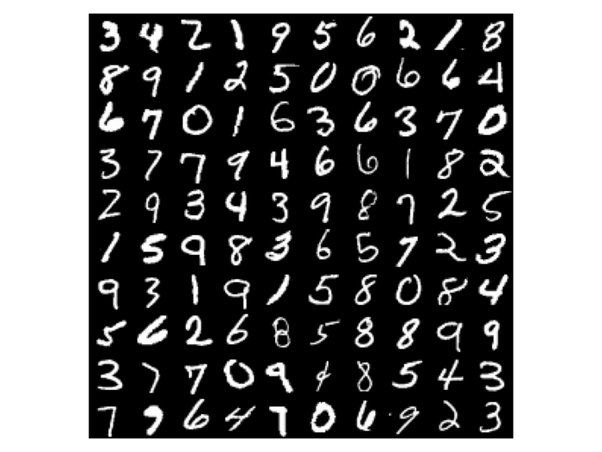
\includegraphics[width=8cm,height=8cm]{imgs/mnist.jpeg}};


\pic[shift={(3,0,0)}] at (input) 
    {Box={
        name=conv1,
        caption=Conv + ReLU,
        xlabel={{1, }},
        zlabel=32,
        fill=\ConvColor,
        height=20,
        width=2,
        depth=20
        }
    };


\draw [connection]  (input) ++(0,0,0)    -- node {\midarrow} (conv1-west);


\pic[shift={(2,0,0)}] at (conv1-east) 
    {Box={
        name=conv2,
        caption=Conv + ReLU,
        xlabel={{32, }},
        zlabel=64,
        fill=\ConvColor,
        height=12,
        width=4,
        depth=12
        }
    };


\draw [connection]  (conv1-east)    -- node {\midarrow} (conv2-west);


\pic[shift={(2,0,0)}] at (conv2-east) 
    {Box={
        name=conv3,
        caption=Conv + ReLU,
        xlabel={{64, }},
        zlabel=128,
        fill=\ConvColor,
        height=6,
        width=6,
        depth=6
        }
    };


\draw [connection]  (conv2-east)    -- node {\midarrow} (conv3-west);


\pic[shift={(2,2,0)}] at (conv3-east) 
    {Box={
        name=fcn1,
        caption=FC + ReLU,
        xlabel={{" ","dummy"}},
        zlabel=32,
        fill=\SoftmaxColor,
        opacity=0.8,
        height=3,
        width=3,
        depth=6
        }
    };


\pic[shift={(2,-2,0)}] at (conv3-east) 
    {Box={
        name=fcn2,
        caption=FC + ReLU,
        xlabel={{" ","dummy"}},
        zlabel=32,
        fill=\SoftmaxColor,
        opacity=0.8,
        height=3,
        width=3,
        depth=6
        }
    };


\draw [connection]  (conv3-east)    -- node {\midarrow} (fcn1-west);


\draw [connection]  (conv3-east)    -- node {\midarrow} (fcn2-west);


\pic[shift={(2,-2,0)}] at (fcn1-east) 
    {Box={
        name=conv4,
        caption=Conv + ReLU,
        xlabel={{128, }},
        zlabel=64,
        fill=\ConvColor,
        height=6,
        width=6,
        depth=6
        }
    };


\draw [connection]  (fcn1-east)    -- node {\midarrow} (conv4-west);


\draw [connection]  (fcn2-east)    -- node {\midarrow} (conv4-west);


\pic[shift={(2,0,0)}] at (conv4-east) 
    {Box={
        name=conv5,
        caption=Conv + ReLU,
        xlabel={{64, }},
        zlabel=32,
        fill=\ConvColor,
        height=12,
        width=4,
        depth=12
        }
    };


\draw [connection]  (conv4-east)    -- node {\midarrow} (conv5-west);


\pic[shift={(2,0,0)}] at (conv5-east) 
    {Box={
        name=conv6,
        caption=Conv + ReLU,
        xlabel={{32, }},
        zlabel=32,
        fill=\ConvColor,
        height=20,
        width=2,
        depth=20
        }
    };


\draw [connection]  (conv5-east)    -- node {\midarrow} (conv6-west);


\pic[shift={(2,0,0)}] at (conv6-east) 
    {Box={
        name=conv7,
        caption=Conv + ReLU,
        xlabel={{32, }},
        zlabel=1,
        fill=\ConvColor,
        height=20,
        width=2,
        depth=20
        }
    };


\draw [connection]  (conv6-east)    -- node {\midarrow} (conv7-west);


\node[canvas is zy plane at x=3] (output) at (conv7-east) {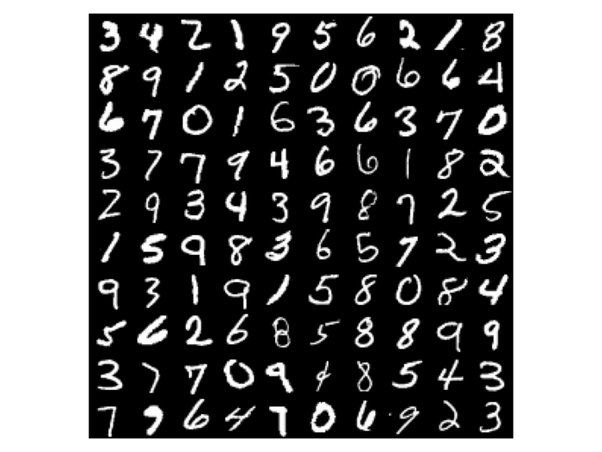
\includegraphics[width=8cm,height=8cm]{imgs/mnist.jpeg}};


\draw [connection]  (conv6-east)     -- node {\midarrow} ($(output) + (0.5,0,0)$);


\end{tikzpicture}
}
    \caption[Architecture of the VAE used for horizontal self-organisation with bigger field-of-view up-sampling]{Architecture of the variational auto-encoder used for horizontal self-organisation with bigger field-of-view up-sampling.}
    \figlbl{horizontal_org_arch2}
\end{figure}

When using $4$ VAEs, the input is divided into $4$ patches. But if the decoder makes the output twice as large as the input by up-sampling, then the entire image is predicted. Thus, in the case of this architecture with $4$ VAEs, the task is to predict the entire image based on a patch that is only a quarter of the image. This is visualized in \figref{bigger_patches}.

\begin{figure}[h]
    \centering
    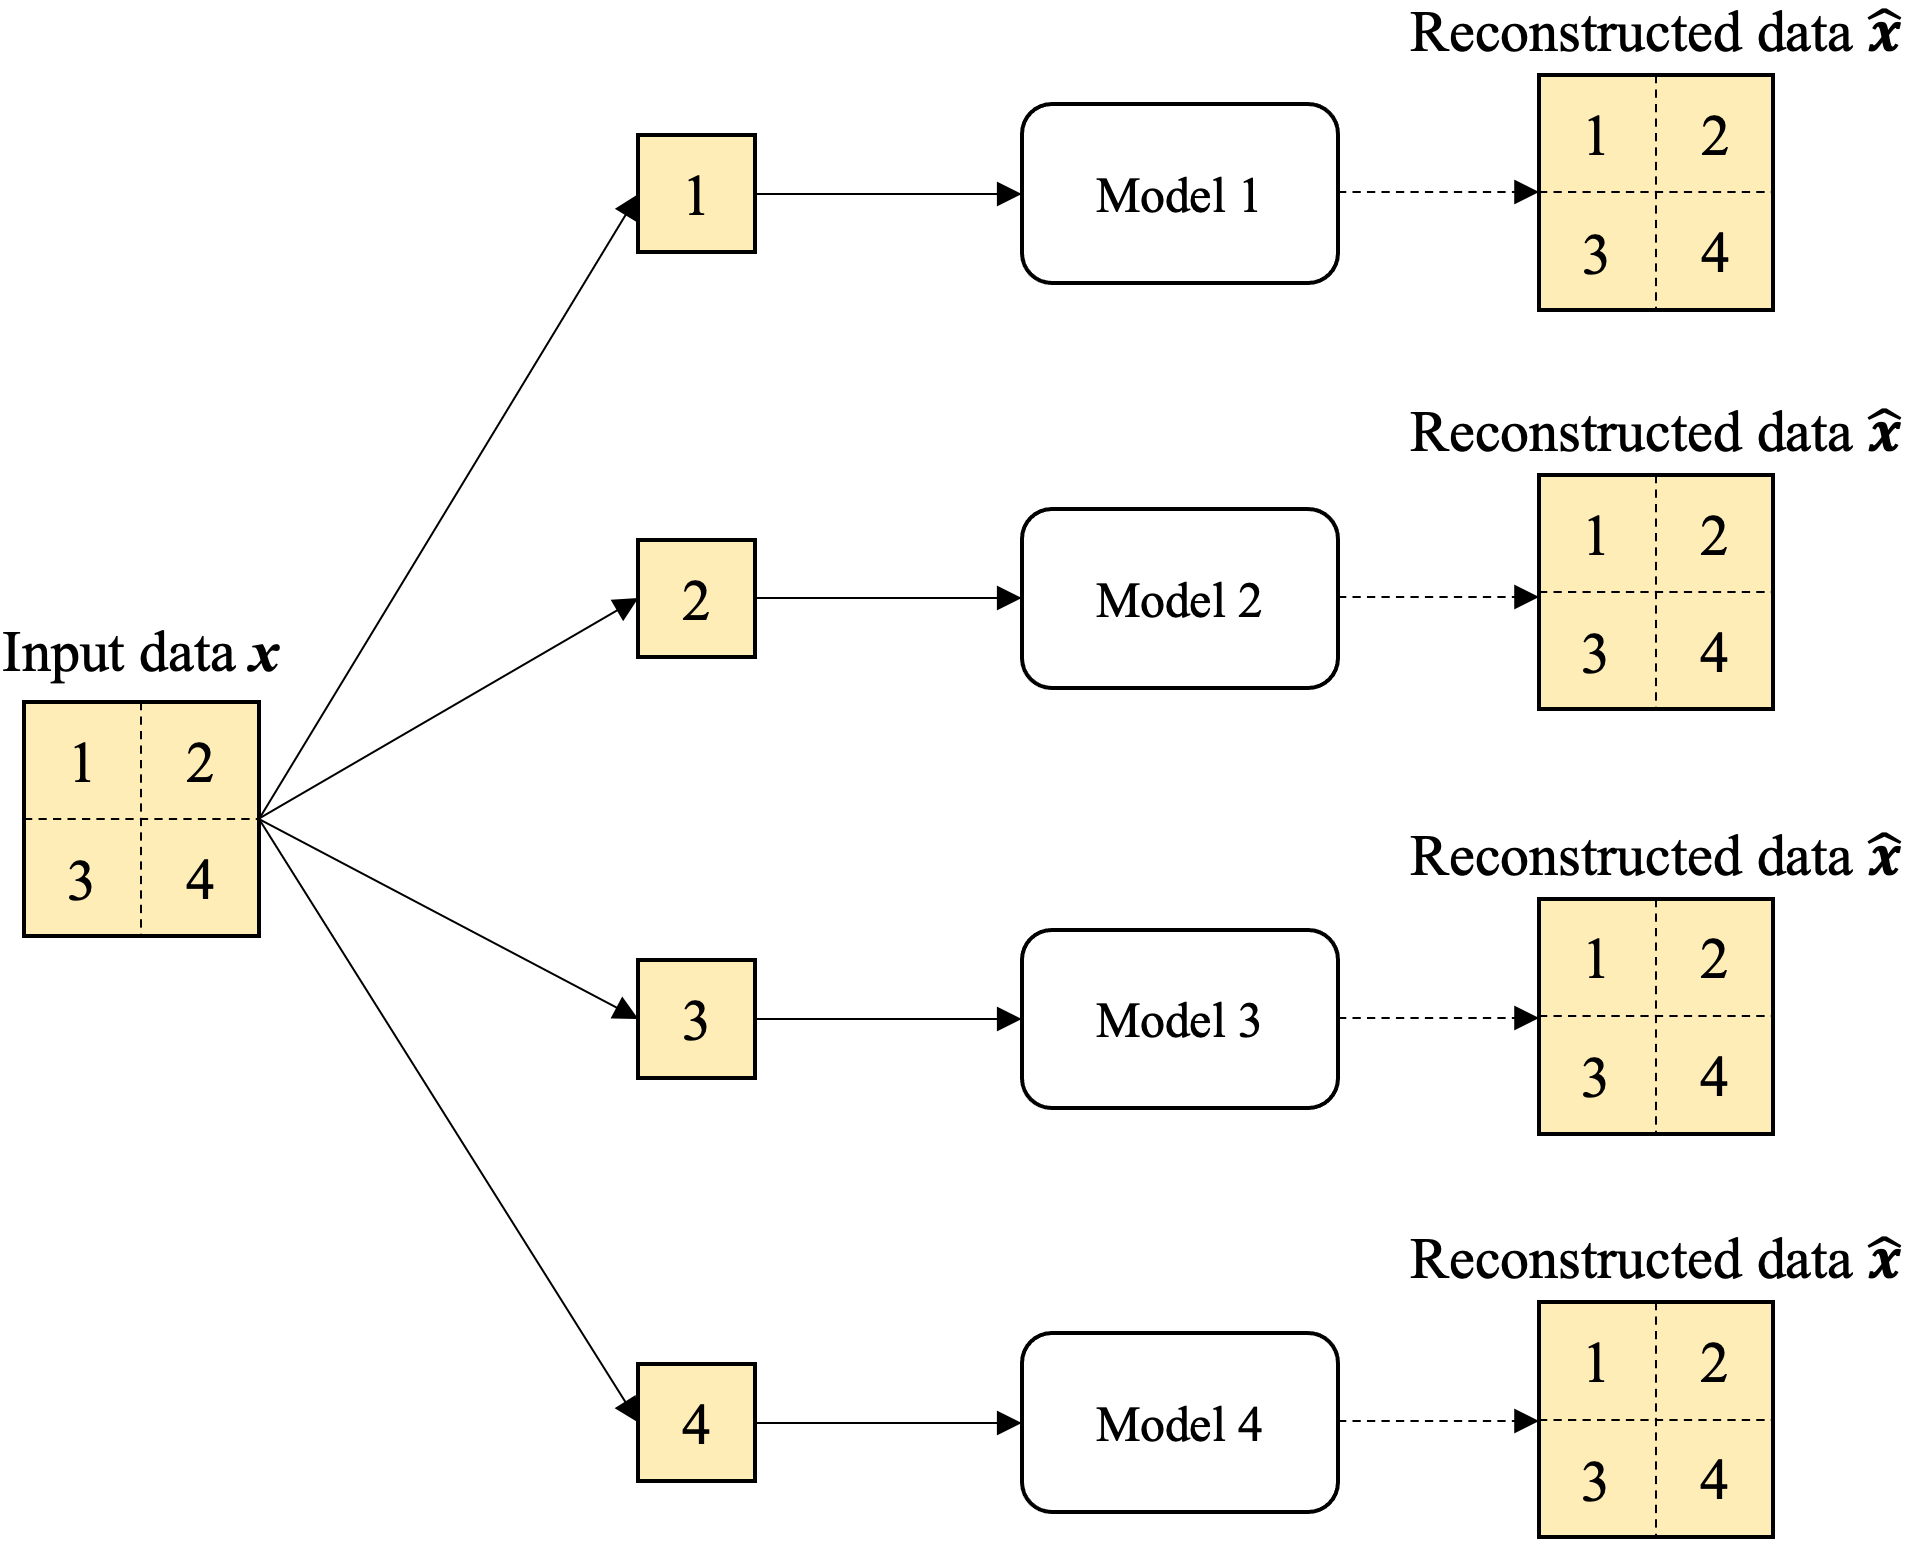
\includegraphics[width=0.99\textwidth]{bigger_patches}
    \caption[Reconstruction of bigger output than input patches]{Four models receive a quarter of the image as input patch to predict the entire image.}
    \figlbl{bigger_patches}
\end{figure}


\subsection{Communication}\seclbl{horizontal_self_org_methods_communication}
The VAEs receive patches of the input image and thus have a very limited field-of-view on the image.
Figure \figref{average_sample} visualizes the patches that are fed into the VAEs when the MNIST data set \cite{Lecun_Bottou_Bengio_Haffner_1998} is used.
The first row shows the average over all images of the same class. Thus, this images are rather representative for the data set.
However, none of the models receives the entire image as input. Instead, the patches shown in 2nd to the 5th row are fed into the VAEs.
The patches, which only depict a quarter of the image, look rather similar for some classes. For example, the top-left patches of the classes $0$ and $9$, as well as the classes $4$, $5$, and $6$ look very similar.
This means that these classes are placed at the same location in the latent space and thus are not separable by \emph{one} single VAE on its own.
Therefore, communication with neighbouring models is necessary to agree on an image representation.

\begin{figure}[h]
    \centering
    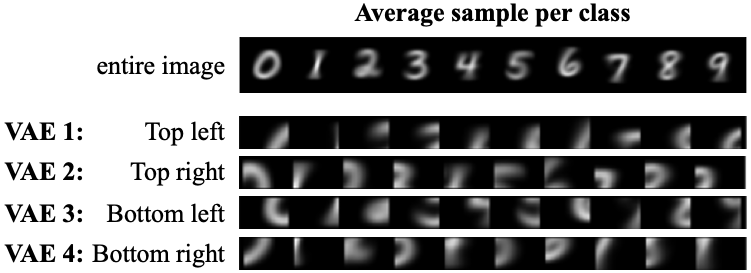
\includegraphics[width=0.99\textwidth]{average_sample}
    \caption[Average sample of the MNIST data set per class]{The average of all samples in the MNIST data set for each class. The first row shows the average of all samples, the 2nd to 5th row the average per patch that is fed into the models.}
    \figlbl{average_sample}
\end{figure}

This connection maps well to the biological model: The single VAEs can be seen as neurons or neuron groups. At the beginning, they have many suggestions as to which classes the patch they read could belong to. Through communication with neighbouring VAEs, however, certain suggestions are constantly ruled out because they are not supported by neighbouring VAEs. Thus, out of many suggestions, only the most valid ones are retained, resulting in an image representation. The biological model behaves similarly: At first, many neurons are active because they are excited by the captured image. However, this strong activation is quickly becoming sparse as only the neurons that support each other remain active. This leads to the emergence of higher-level features (i.e. net fragments) that are representative for the captured input.


TODO: add source from Christoph


Thus, the communication between VAEs is a lateral support of representations. This corresponds to the lateral connections introduced in section \secref{lateral_connections}: Each VAE (which can be interpreted as a neuron) makes several suggestions as to what the patch could represent. Only the representations that are laterally supported are retained and the other representations are discarded. To learn representations in an unsupervised manner (and to keep one of the strengths of auto-encoders), no probability of predefined labels should not be communicated as this requires label information. Instead, different types of communication are proposed that work without labels: communication based on the latent representations, communication based on the reconstructed images, and communication via a dedicated communication channel.

All these types of communication take place over two or more time-steps. First, image patches are reconstructed by all VAEs. As a result, each VAE generates information in latent space. This information can be communicated to the neighbouring VAEs. Thus, in a second time-step, the VAEs have more information at available: their own prediction based on the reconstructed image patch and information from neighbouring VAEs. This additional information allows them to improve their own prediction. The process can be repeated either over a fixed number of time-steps or until the network reaches an attractor state (i.e. the latent representations do not change anymore).


\subsubsection{Model Heads}
Each VAE learns the mapping from a patch to a latent space with Gaussian distribution, i.e. obtains a $\boldsymbol{mu}$ and $\boldsymbol{sigma}$ for each sample that is used to predict a reconstructed version of the input.
The arrangement of the representations within the latent space is not predetermined by an external system but is formed by the model itself in the manner of self-organisation. A consequence of this is that $\boldsymbol{mu}$ and $\boldsymbol{sigma}$ have a different meaning in the latent spaces of different VAEs. Thus, one VAE is not able to interpret the Gaussian parameters of another VAE out-of-the-box.

In this thesis, we propose to learn a linear transformation to map the Gaussian parameters of one VAE to the Gaussian parameters of another VAE. The mapping from $\boldsymbol{mu}_1$ to $\boldsymbol{mu}_2$, respectively from $\boldsymbol{sigma}_1$ to $\boldsymbol{sigma}_2$ is done by the simple transformation

\begin{equation}\eqlbl{hso_7}
	\boldsymbol{\hat{\mu}}_2 = \boldsymbol{w}_{m12} \cdot \boldsymbol{\mu}_1
\end{equation}

resp.

\begin{equation}\eqlbl{hso_8}
	\boldsymbol{\hat{\sigma}}_2 = \boldsymbol{w}_{s12} \cdot \boldsymbol{\sigma}_1
\end{equation}

The weights $\boldsymbol{w}_{mij}$ and $\boldsymbol{w}_{sij}$ between VAE $i$ and VAE $j$ are learned by minimising the mean square error with gradient descent between the predicted and true Gaussian parameters, i.e. between $\boldsymbol{\mu}_j$ and $\boldsymbol{\hat{\mu}}_j$, resp. $\boldsymbol{\sigma}_j$ and $\boldsymbol{\hat{\sigma}}_j$. This process is illustrated for VAE 1 in Figure \figref{hso_head}. First, the Gaussian parameters of each model must be predicted for the same sample. Afterwards, the Gaussian parameters of one model can be used to predict the Gaussian parameters of the other models with a linear transformation.

\begin{figure}[h]
    \centering
    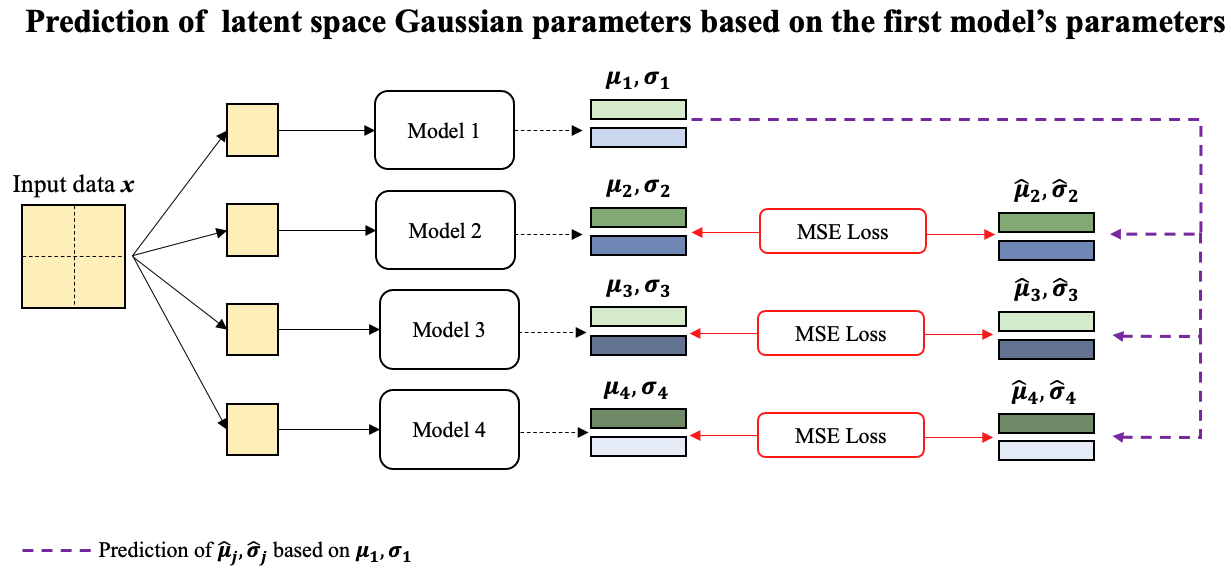
\includegraphics[width=0.99\textwidth]{hso_head}
    \caption[Prediction of Gaussian parameters of other VAEs]{Visualization of how the first VAE can predict the Gaussian parameters of the other VAEs.}
    \figlbl{hso_head}
\end{figure}

This makes it possible to predict the Gaussian parameters of all VAEs on the basis of one patch and to reconstruct the entire image. If each VAE predicts the Gaussian parameters of the other VAEs, then each VAE receives further suggestions from neighbouring VAEs in addition to the parameters calculated by the encoder. Thus, each VAE has its own calculated Gaussian parameters as well as suggestions from neighbours about what its Gaussian parameters might be. This allows a VAE to correct its prediction. This is particularly interesting because the suggestions made by neighbouring VAEs are based on a different patch. For example, the VAE that sees only one patch from the top left of the image cannot distinguish the digits $5$ and $6$. The VAE that sees the patch at the bottom left, on the other hand, is able to distinguish these digits. Thus, the VAE at the bottom left can help the VAE at the top left to choose a better latent representation.

TODO: At the moment, various experiments are still ongoing to find out how this can be implemented (therefore, not yet explained in more detail).


\subsubsection{Reconstructed Images}
As described in \secref{horizontal_self_org_methods_bigger_patches}, the prediction of larger patches helps to better arrange the latent space. The prediction of larger patches can also be used for communication with neighbouring VAEs. Instead of extracting representations from the latent space and transmitting them to neighbouring VAEs as described in the last section, the reconstructed image can also be exchanged. This is done by predicting a part of the image in a first time-step and by adding this prediction to an additional input channel of another VAE in the next time-step. Various data can be forwarded to other VAEs:% and is explained below. Let $\boldymbol{x}$ be the input image and $\boldymbol{\hat{x}}$ the reconstructed image. For $n$ VAEs, the input sample $\boldymbol{x}$ is split into $n$ non-overlapping patches $\boldymbol{x}^{(1)}, ..., \boldymbol{x}^{(n)}$. The reconstructed patches are denoted as $\boldymbol{\hat{x}}^{(1)}, ..., \boldymbol{\hat{x}}^{(n)}$. If a VAE reconstructs the same patch as it received as input, $\boldymbol{x}^{(i)} \approx \boldymbol{\hat{x}}^{(i)}$ is valid. However, when a bigger patch is predicted than the one that was fed into the model, then this term is not valid anymore, i.e. $\boldymbol{x}^{(i)} \not\approx \boldymbol{\hat{x}}^{(i)}$. However, if only a part of the prediction $\boldymbol{\hat{x}}^{(i)}$ is considered (i.e. the prediction is cropped), then $\boldymbol{x}^{(i)}$ is contained in this cropped version of the prediction $\boldymbol{\hat{x}}^{(i)}_C$.


\begin{figure}
    \centering
    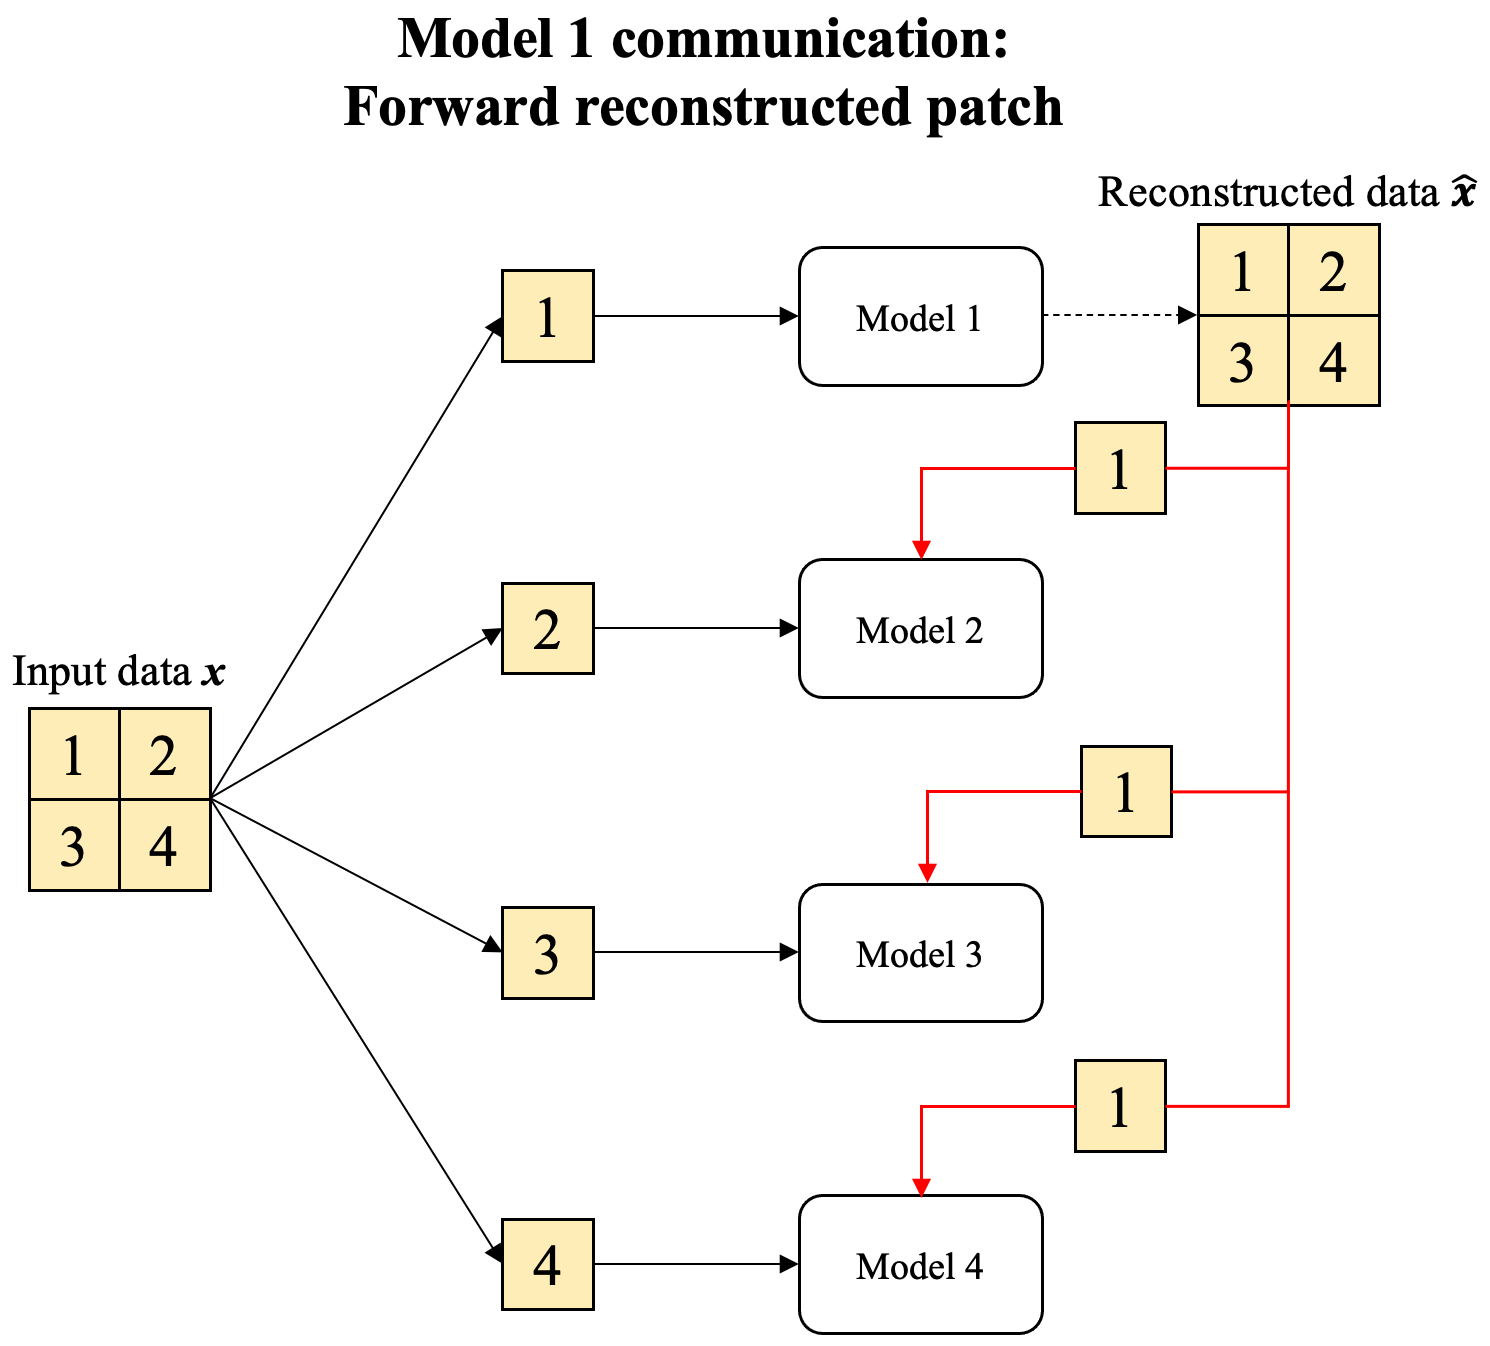
\includegraphics[width=0.80\textwidth]{recon_patch_forw}
    \caption[Communication between VAEs by forwarding reconstructed patch]{Communication between VAEs by forwarding reconstructed patch, example on the basis of the first VAE: The first VAE predicts the image and forwards the reconstructed patch (the same patch that was fed into the model) to the other VAEs.}
    \figlbl{recon_patch_forw}
\end{figure}

\begin{figure}
    \centering
    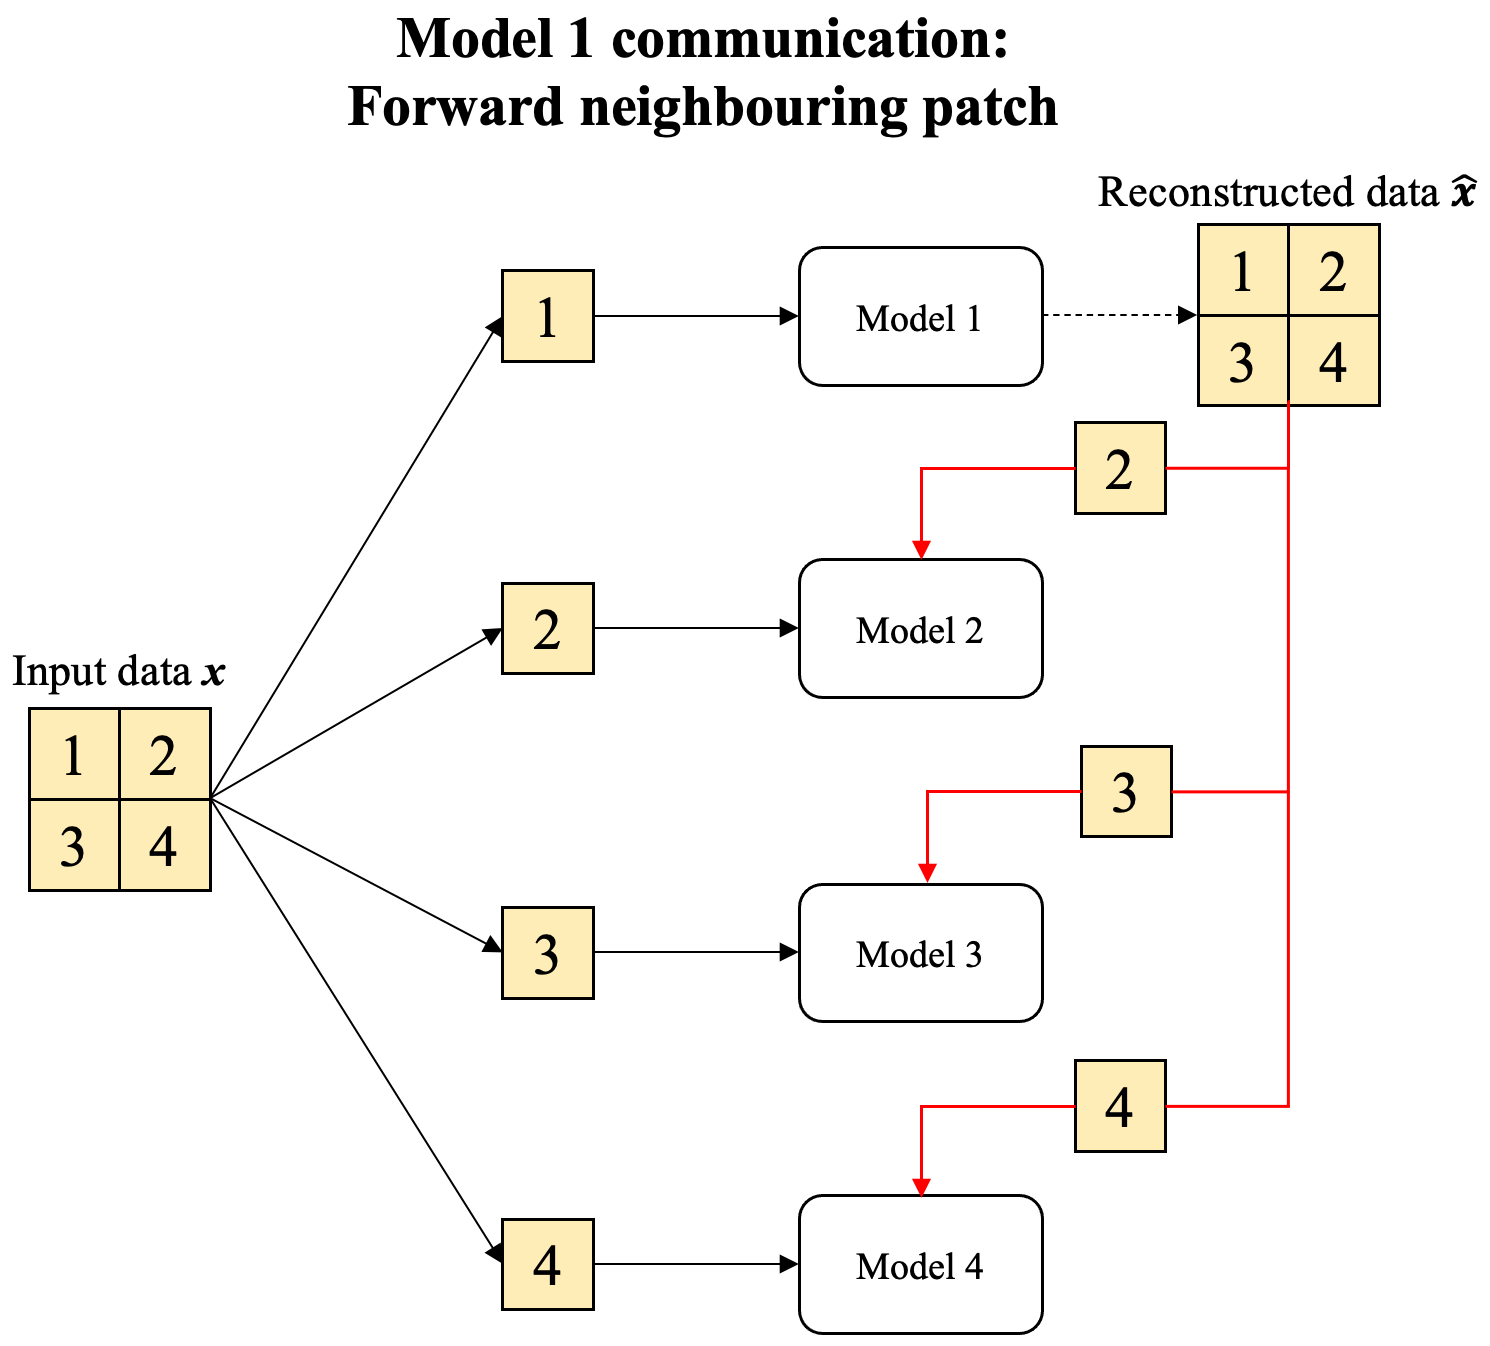
\includegraphics[width=0.80\textwidth]{neighbouring_patch_forw}
    \caption[Communication between VAEs by forwarding prediction of neighbouring patches]{Communication between VAEs by forwarding prediction of neighbouring patches, example on the basis of the first VAE: The first VAE predicts the image and forwards a prediction of how the neighbourhood could look like to the other VAEs. Thus, each other VAE receives a patch and a prediction of the first VAE how this patch could look like as input.}
    \figlbl{neighbouring_patch_forw}
\end{figure}

\begin{figure}
    \centering
    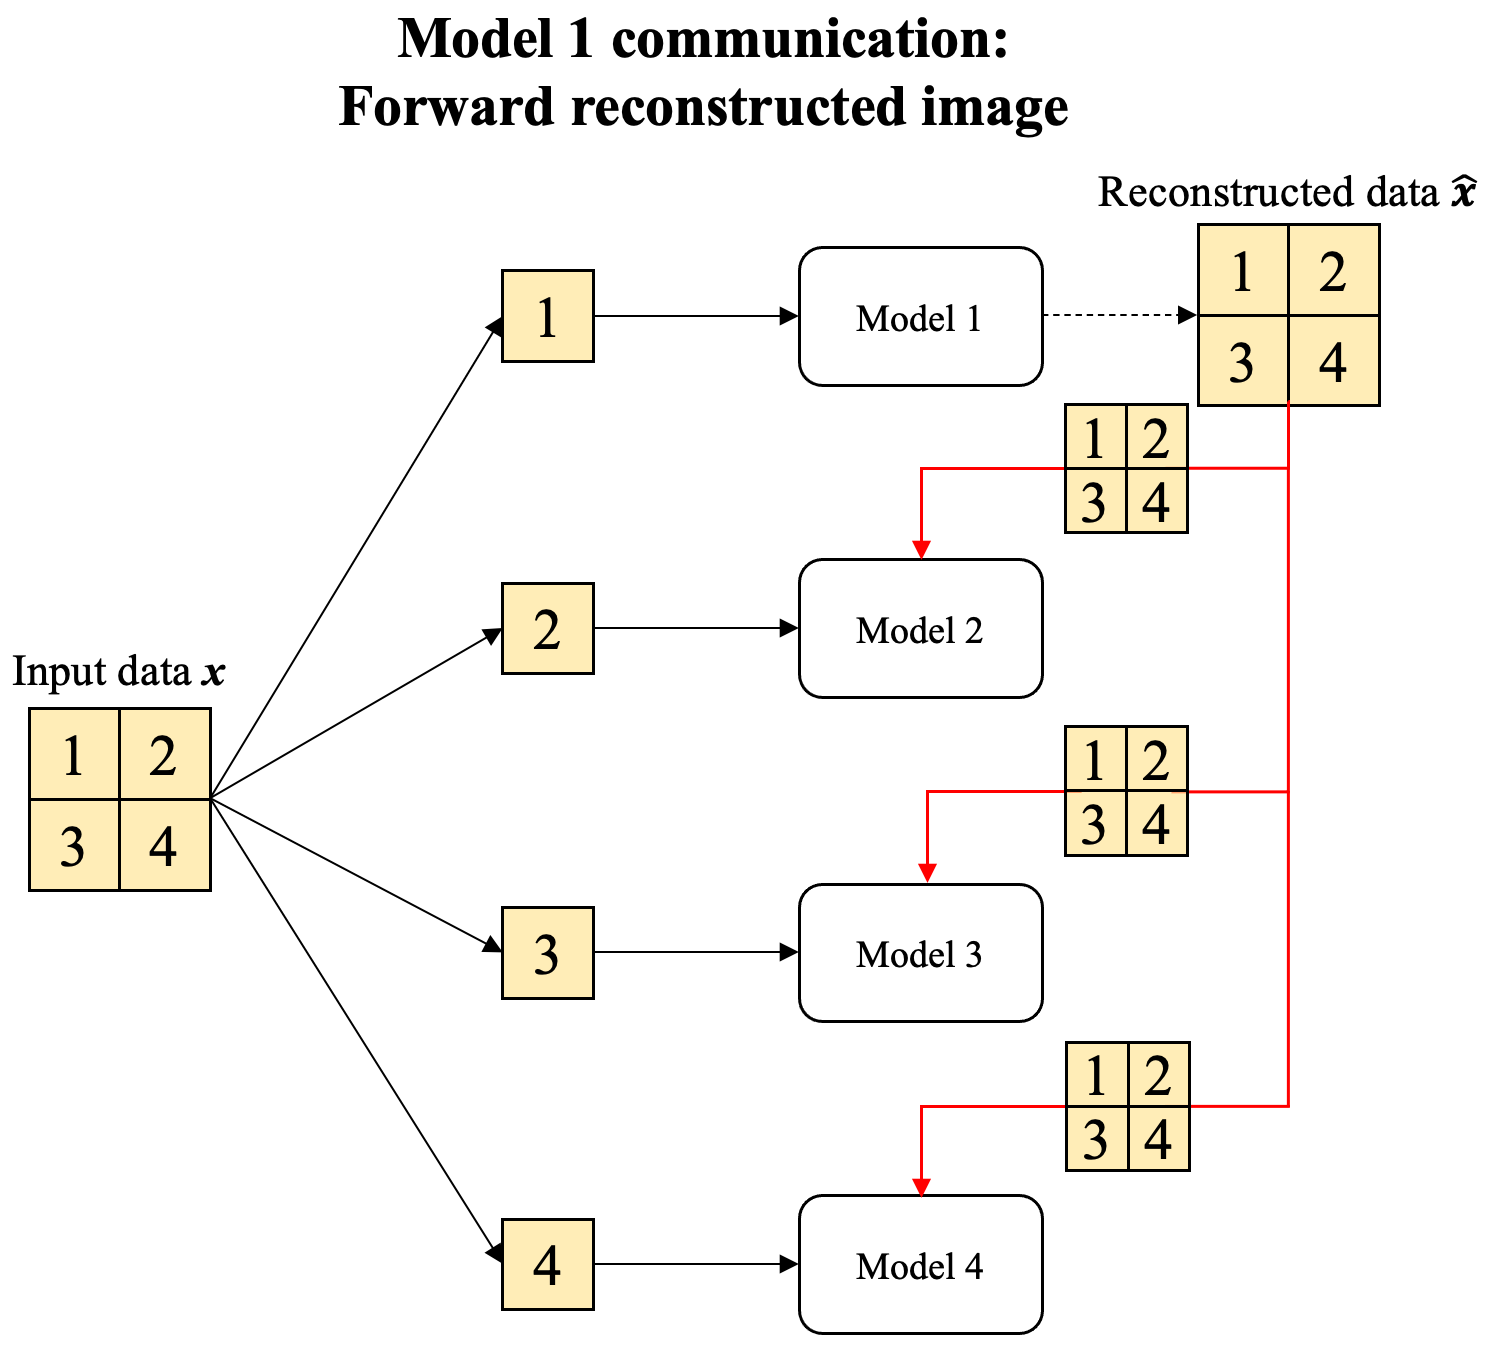
\includegraphics[width=0.80\textwidth]{recon_img_forw}
    \caption[Communication between VAEs by forwarding prediction of the entire image]{Communication between VAEs by forwarding prediction of the entire image, example on the basis of the first VAE: The first VAE predicts the image and forwards the prediction of the image to the other VAEs.}
    \figlbl{recon_img_forw}
\end{figure}



\begin{description}
	\item [Reconstructed Patch] Each VAE reconstructs its input patch and optionally a part of the neighbourhood. It tells the other VAEs what the reconstructed version of its input patch looks like. Information about the optionally reconstructed neighbourhood is not communicated to other VAEs. Thus, a reconstructed version of the input is sent to other VAEs and added as a new channel to their input. This process is exemplified for the first VAE in \figref{recon_patch_forw}. The problem with this approach is that in the first time-step all VAEs reconstruct their patch and the reconstructed version is communicated to the neighbouring VAEs. As a result, in the second time-step, each VAE receives information about the entire image and thus has access to global instead of only local image information\sidenote{even with a very large number of VAEs and communication restricted to the local neighbourhood, information about the entire image propagates to all VAEs over time, provided enough time-steps are executed}.  
	\item [Neighbouring Patch] Instead of communicating the reconstructed input patch to the neighbours, a prediction can be made of what the input patch of the neighbour looks like and this prediction can be communicated. This has the advantage that each UAE receives different versions of the same patch as input and thus has no global image information. This process for the first VAE is visualised in \figref{neighbouring_patch_forw}. Intuitively, this can solve the following problem: If a VAE cannot decide which digit to predict, neighbouring VAEs can help it by predicting its input patch in a form that is more similar to one of the digits and thus support the VAE by making its decision. 
	\item[Entire image] The simplest version is when each VAE predicts the entire image and communicates this to all other VAEs. In the first time-step, only local information is available, in the second time-step, various predictions of how the image could look are additionally provided. Each VAE can then correct its own prediction based on these predictions of the other VAEs. This process is represented in \figref{recon_img_forw}. Identical to ``reconstructed patches'', global image information is made available to each VAE. This problem can be alleviated if for each VAE $i$ that receives the input patch $\boldsymbol{x}^{(i)}$, the part from its prediction of the whole image corresponding to $\boldsymbol{x}^{(i)}$ is masked. Otherwise, an input patch of a VAE is fed through the encoder and decoder and then communicated to the other VAEs. Then implicitly reconstructed data and not just neighbourhood predictions gets to each VAE as input. 
\end{description}



\subsubsection{Communication Channel}
Another way to communicate is through a dedicated communication channel. For this purpose, each VAE has not only $1$ input and $1$ output channel but $4$ input and output channels. The input patch is fed into the first channel and a reconstructed version of it is predicted in the first output channel. This corresponds to a classic VAE and the loss function remains identical.
The remaining three channels are for communication: Each VAE generates a separate communication output for its $3$ neighbouring VAEs on the remaining $3$ channels. Each of these channels is then stacked to the input of the corresponding VAE. For example, the first VAE receives a given patch on the input channel $1$ and communication data from the 2nd, 3rd, and 4th VAE on the input channels $2$-$4$. Based on this information, it outputs a reconstruction of the patch on the output channel $1$ and communication data to the 2nd, 3rd, and 4th VAE on the output channels $2$-$4$. Thus, there is a dedicated two-way communication channel between each neighbouring VAE. This is shown in \figref{vae_comm_channel}.


\begin{figure}[h]
    \centering
    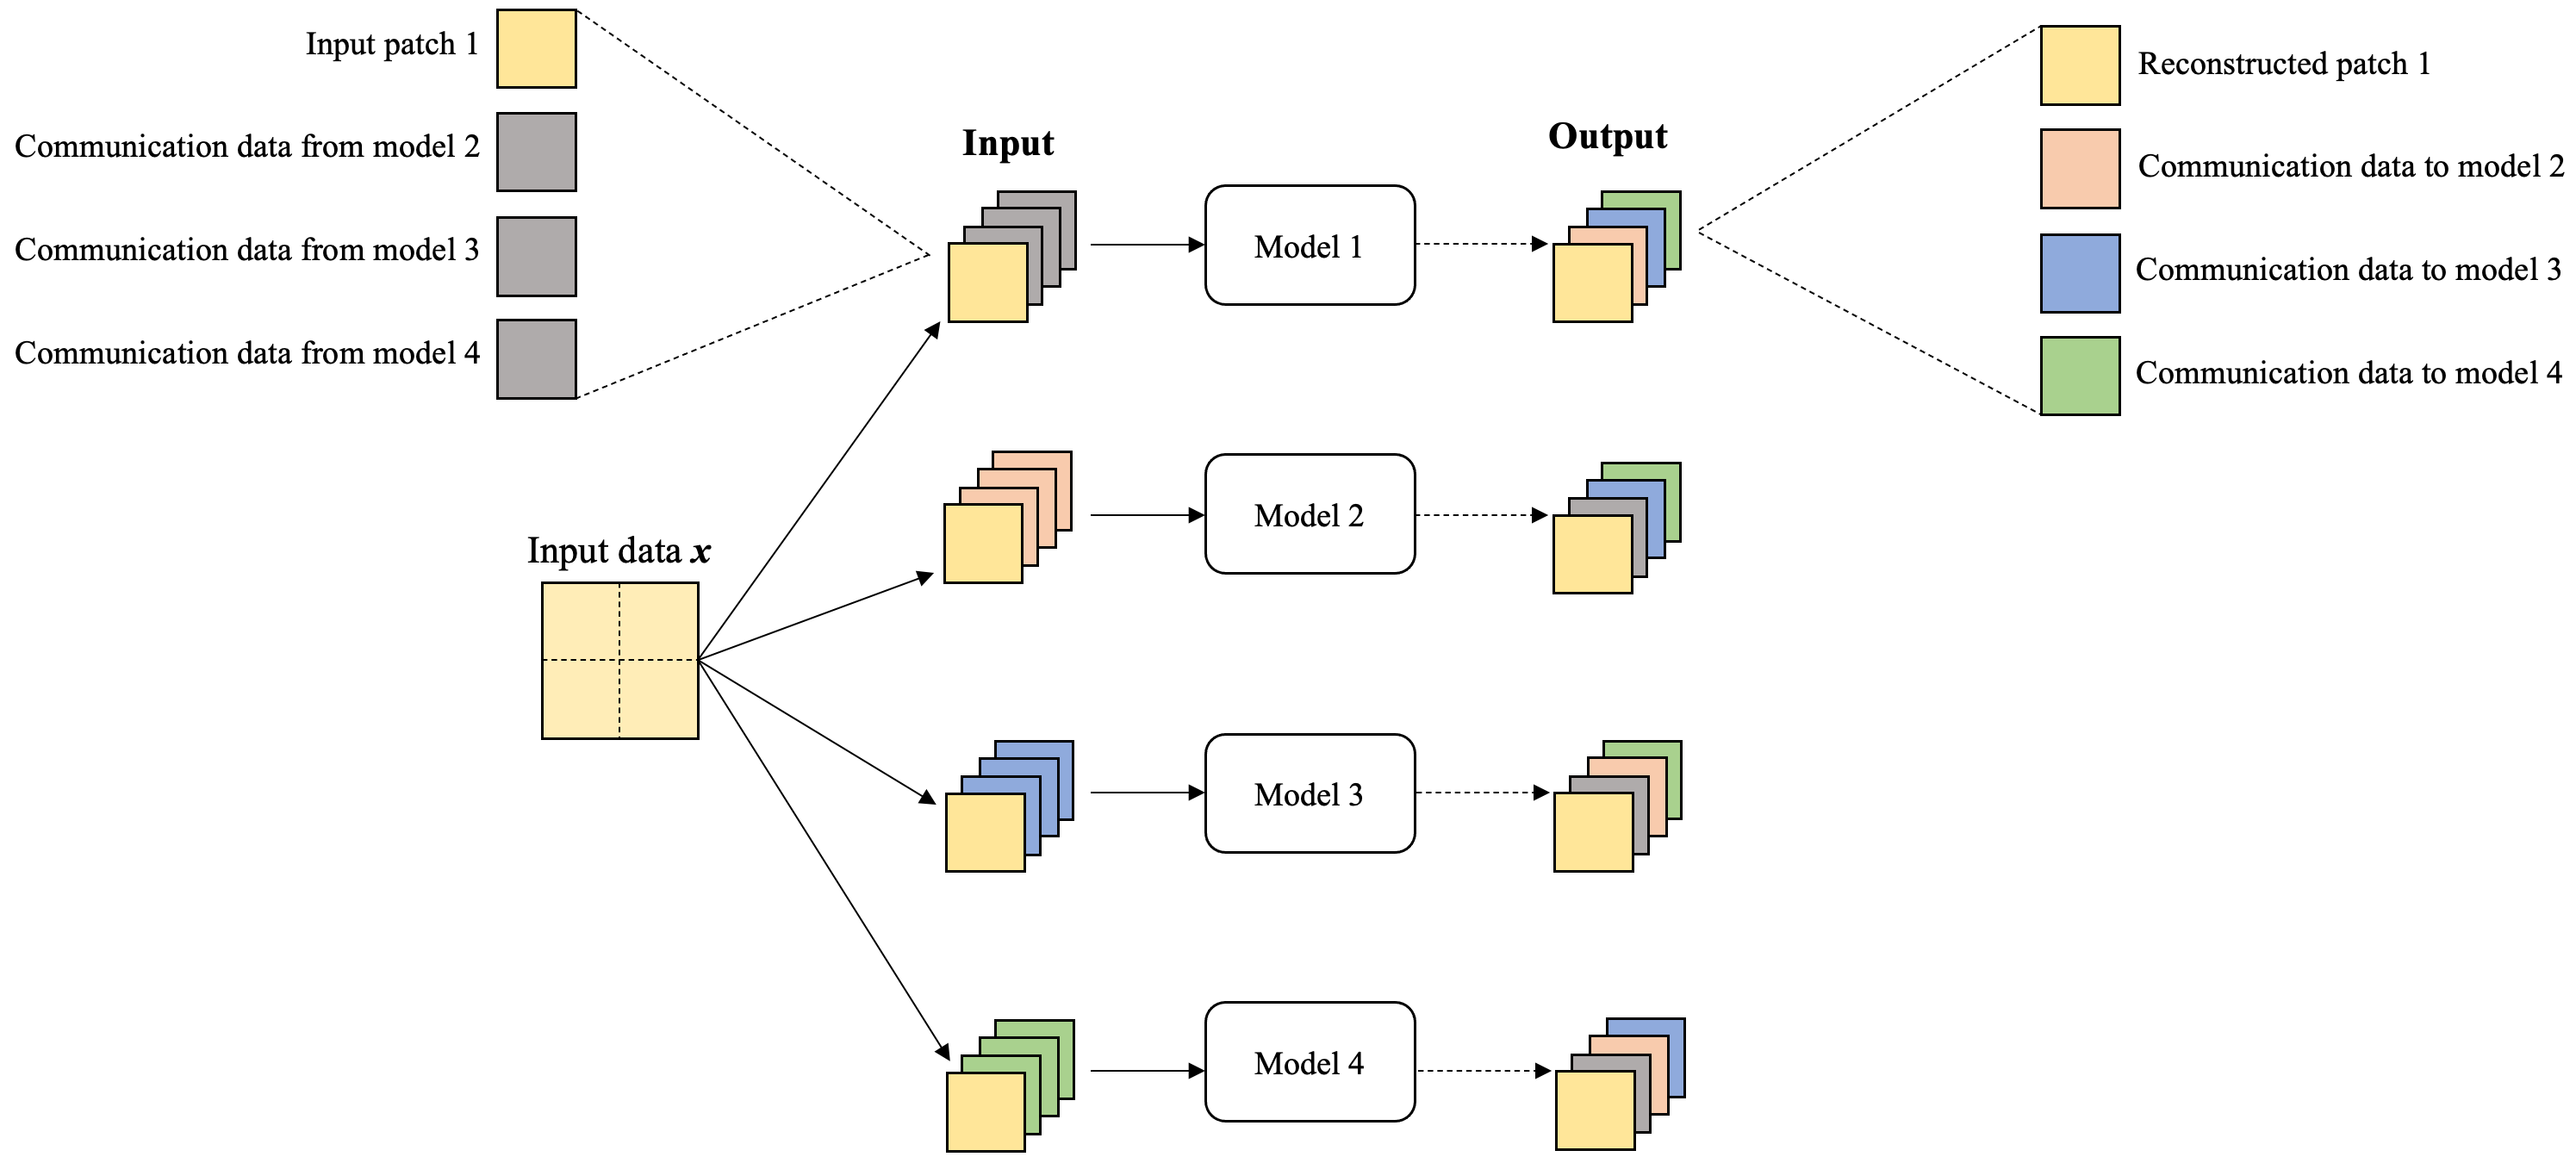
\includegraphics[width=0.89\textwidth]{vae_comm_channel}
    \caption[Communication between VAEs with a dedicated communication channel]{Each VAE has one and output channel to receive and reconstruct a given image patch. The other input and output channels are used for communication: Each VAE has for each other VAE a separate output channel to send messages and an additional input channel to receive messages.}
    \figlbl{vae_comm_channel}
\end{figure}

The loss function remains the same for the first output channel since the goal is still the same, i.e. to reconstruct the output as good as possible. The only difference is that model can now access $4$ input channels to reconstruct the input instead of one channel. However, the communication channels must be trained in order for them to be helpful for input reconstruction. Therefore, an additional loss term is applied on the $3$ output communication channels. Thereby, the idea is to optimize the output of these communication channels in a way so that the other VAEs can better reconstruct their patch.

Let $V = {V_1, ..., V_n}$ be the set of $n$ VAEs. Each VAE has $n$ output channels, one channel for the reconstructed image and $n-1$ channels for communication. Furthermore, each VAE $V_i$ has a loss $L_{\text{VAE}_i}$ based on the reconstruction goodness and the shape of the latent space (c.f. \eqref{hso_6}). The $3$ communication channels of a VAE $i$ can influence the loss $L_{VAE_j}$ of VAE $j$ (i.e. help to improve the loss by providing better information). How helpful the communication channels are can therefore be determined by the average of the loss of the other VAEs.

\begin{equation}\eqlbl{hso_9}
	L_{c_i} = \frac{1}{n-1} \sum_{n}^{j=1} L_{\text{VAE}_j} \text{, if } i \neq j
\end{equation}

Thus, the loss of a VAE with communication channel is

\begin{equation}\eqlbl{hso_10}
		L_{{\text{VAE}_C}_i} = L_{\text{VAE}_i} + \beta \cdot L_{\text{KLD}_i} + \beta_2 \cdot L_{c_i}
\end{equation}

where $\beta_2$ is a weight factor for the communication channel. Thus, each model optimizes its own reconstruction error, the shape of the latent space, and tries to improve the latent space and reconstruction error of other VAEs.


TODO: This has not been implemented yet (therefore, not explained in more detail).


\subsection{Class Prediction}
The VAEs are examined whether they are suitable for predicting the class label. To do this, all VAEs are first trained until they can reliably reconstruct images and the latent space is well formed.
After training, the average value of $\boldsymbol{\mu}$ is determined for each class $c \in C$ from the training set and each VAE $v$. This average value is called $\boldsymbol{\mu}_{\text{avg}_c}$ and is defined for $n$ samples as

\begin{equation}\eqlbl{hso_12}
		\boldsymbol{\mu}_{\text{avg}_vc} = \frac{1}{n} \sum_{i=1}^{n} \boldsymbol{\mu}_i
\end{equation}

This average value can be considered as the ``cluster centre'' of a class in latent space. In addition, $\boldsymbol{\mu}_{\text{avg}_vc}$ is a world model of a class. To make a prediction, a given sample is matched against these world models per class. As with vertical self-organisation, the cosine similarity between a sample and the class prototypes is used to determine their similarity. To predict a sample, first its $\boldsymbol{\mu}_vs$ is determined. Then, this sample is compared with all classes by computing the cosine similarity: 

\begin{equation}\eqlbl{hso_13}
		\text{cos}_{vsc} = \text{cos}(\boldsymbol{\mu}_vs, \boldsymbol{\mu}_{\text{avg}_vc}) = \frac{\boldsymbol{\mu}_vs \cdot \boldsymbol{\mu}_{\text{avg}_vc}}{\max(||\boldsymbol{\mu}_vs||_2, ||\boldsymbol{\mu}_{\text{avg}_vc}||_2)}
\end{equation}

Thus, the cosine similarity $\text{cos}_{vsc}$ between each class $c$' prototype and the sample $s$ is calculated for each VAE $v$.
Afterwards, the average class $c$ with the highest average cosine similarity between the sample activations $\boldsymbol{\mu}_vs$ and the class prototypes $\boldsymbol{\mu}_{\text{avg}_vc}$ is used as prediction.

\begin{equation}\eqlbl{hso_14}
		\argmax_{c \in C} \frac{1}{4} \sum_{v=1}^{4} \text{cos}_{vsc}
\end{equation}

Similar to vertical self-organisation, VAE's with a higher confidence have a higher cosine similarity between a class prototype and a specific class and thus have more influence on the class prediction than if the confidence is lower and the cosine similarity between the sample and all class prototypes is similarly large.

TODO: This has to be improved by also considering the standard deviation


TODO: Another improvement is to use multiple prototypes per class as digits may be written differently (depending on the person) and thus look different


\subsubsection{VQ-VAE}
In the case of classification, the latent space has to be shaped in a way that allows to assign a latent representation to a class.
This can be simplified if the encoder maps the input image to a discrete variable in the latent space.
Vector quantised variational auto-encoders (VQ-VAE) \sidecite{NIPS2017_7a98af17} model such a discrete latent space by using vector quantisation (VQ).
Vector quantisation is a method that maps multi-dimensional vectors to a finite set of ``code''-vectors.
An image is fed into the encoder to obtain the encoder output $\boldsymbol{z}_e$.
Afterwards, a nearest neighbour lookup is made to find the code-vector that is most similar to $\boldsymbol{z}_e$.
The code-vector, also called the quantized vector $\boldsymbol{z}_q$ is fed into the decoder to reconstruct the image.


TODO: This has not been implemented yet (therefore, not explained in more detail).


\section{Results}\seclbl{horizontal_self_org_results}
As for vertical self-organisation (.c.f \secref{vertical_self_org_methods_dataset}), the MNIST data set is used to evaluate the models. 


% Accuracy 1 VAE: 0.8537

% Accuracy 4 VAE ohne Kommunikation:
%accuracy: 0.8140
%|	 accuracy vae 0: 0.5954
%|	 accuracy vae 1: 0.6578
%|	 accuracy vae 2: 0.6547
%|	 accuracy vae 3: 0.6052








%TODO: vereinheitliche Mathe: Was ist underline, was ist hochgestellt in Klammern ($z^{(i)}$) und was ist hochgestellt in eckigen Klammern? Bei NN: Was ist n, was ist m, ... (+ Lernraten Symbol, Loss Symbol, etc.)
%Sind alle Vektoren bold?

% TODO: target function und objective function vereinheitlichen
% TODO: net-fragment or net fragment

